\documentclass{article}
\usepackage[utf8]{inputenc}
\usepackage{polski}
\usepackage[margin=2cm]{geometry}
\usepackage{graphicx}
\graphicspath{ {./images/} }

\title{Historia Wrocławia}
\date{}

\begin{document}

\maketitle
\tableofcontents

\section{Budorigum}
W czasach antycznych na obecnych terenach Wrocławia lub w bliskiej okolicy istniała miejscowość o nazwie Budorigum. Została ona odwzorowana na antycznej mapie Klaudiusza Ptolemeusza z lat 142–147 n.e.\footnote{Claudius Ptolemy: Book II, Chapter 10: Greater Germany (Fourth Map of Europe) (ang.). W: The Geography [on-line]. [dostęp 2010-12-15].} O tym, że miejscowość ta znajdowała się w okolicach Wrocławia, informuje Lexicon Universale\footnote{Johann Jacob Hofmann: Lexicon Universale. W: Universität Mannheim [on-line]. [dostęp 2010-12-15].} oraz wynika to z położenia wśród innych zidentyfikowanych miejscowości Śląska. Część hipotez łączy antyczną osadę Budorigum z samym Wrocławiem, część wskazuje jednak na jej lokalizację w Brzegu lub jego okolicach.

\section{Założenie miasta}
Według tradycji, gród we Wrocławiu został założony przez czeskiego księcia Wratysława (cz. Vratislav I) (panował 915–921). Nazwa miasta pochodzi być może od skróconej formy imienia założyciela (Wrocisław), jednakże ekspansję na teren Śląska mógł przeprowadzić Bolesław I Srogi dopiero po roku 935, dlatego kwestia nazwy miasta jest polem do dalszych interpretacji. Według ostatnich badań nie ma śladu, który by wskazywał na funkcjonowanie wcześniej niż przed 940 rokiem grodu na wrocławskim Ostrowie Tumskim\footnote{K. Jaworski, P. Rzeźnik, Wrocławski Ostrów Tumski we wczesnym średniowieczu, [w:] Civitates principales, Wybrane ośrodki władzy w Polsce wczesnośredniowiecznej (Katalog wystawy), Gniezno 1998, s. 88–94.}. Nie ma więc możliwości, aby Wrocław wcześniej pełnił rolę czeskiego ośrodka administracyjnego\footnote{ Dariusz Andrzej Sikorski, Wczesnopiastowska architektura sakralna (jako źródło historyczne dla dziejów Kościoła w Polsce), Wydawnictwo Poznańskiego Towarzystwa Przyjaciół Nauk, Poznań 2012, ​ISBN 978-83-7654-244-9​, s. 114}. W roku 985 na Ostrowie Tumskim powstał pierwszy gród wybudowany przez Mieszka I\footnote{Edmund Małachowicz, Najnowszy zarys dziejów najstarszego Wrocławia, Wrocław 2000, s. 49.}. W tym też okresie miasto wraz z resztą Śląska przeszło we władanie rodu Piastów.

W 1000 roku na zjeździe gnieźnieńskim cesarz Otton III i Bolesław Chrobry ustanowili w mieście biskupstwo rzymskokatolickie podporządkowane arcybiskupstwu w Gnieźnie. Krótko po tym powstała w obrębie grodu pierwsza katedra romańska. Choć miasto istniało już wcześniej – datę tę traktuje się oficjalnie jako początek jego istnienia – w 2000 roku uroczyście obchodzono tysiąclecie Wrocławia. Z czasem ośrodek urbanistyczny przeniósł się na lewy brzeg Odry w okolice kościoła św. Andrzeja i Magdaleny, a potem około wieku XIII w okolice kościoła św. Elżbiety i dzisiejszego Starego Miasta.

\section{Rozwój (X–XIII wiek)}
\begin{figure}[ht]
\includegraphics[scale=0.2]{Wrocław12th-13thcentury}
\caption{Wrocław w XII–XIII wieku}
\label{fig:figure1}
\end{figure}
Miasto dzieliło dzieje Śląska będąc jego centrum gospodarczym i administracyjnym. Przy osłabieniu władzy Piastów przechodziło w ręce Przemyślidów. Stało się tak m.in. w 1038, gdy w wyniku trwającego od 4 lat antychrześcijańskiego powstania doszło do najazdu czeskiego księcia Brzetysława I, a biskup wrocławski zmuszony był opuścić gród i aż do restytucji biskupstwa w 1051 rezydował najprawdopodobniej w Smogorzewie koło Namysłowa. Z okresu tego pochodzą odkryte we Wrocławiu szczątki świątyni pogańskiej z lat 30. XI wieku. Z Kroniki polskiej Galla Anonima znamy dwóch komesów Wrocławia z drugiej połowy XI w.: Magnusa i Wojsława\footnote{Tadeusz Szumski, 500 zagadek o Wrocławiu, WP, Warszawa 1971.}.
\begin{figure}[ht]
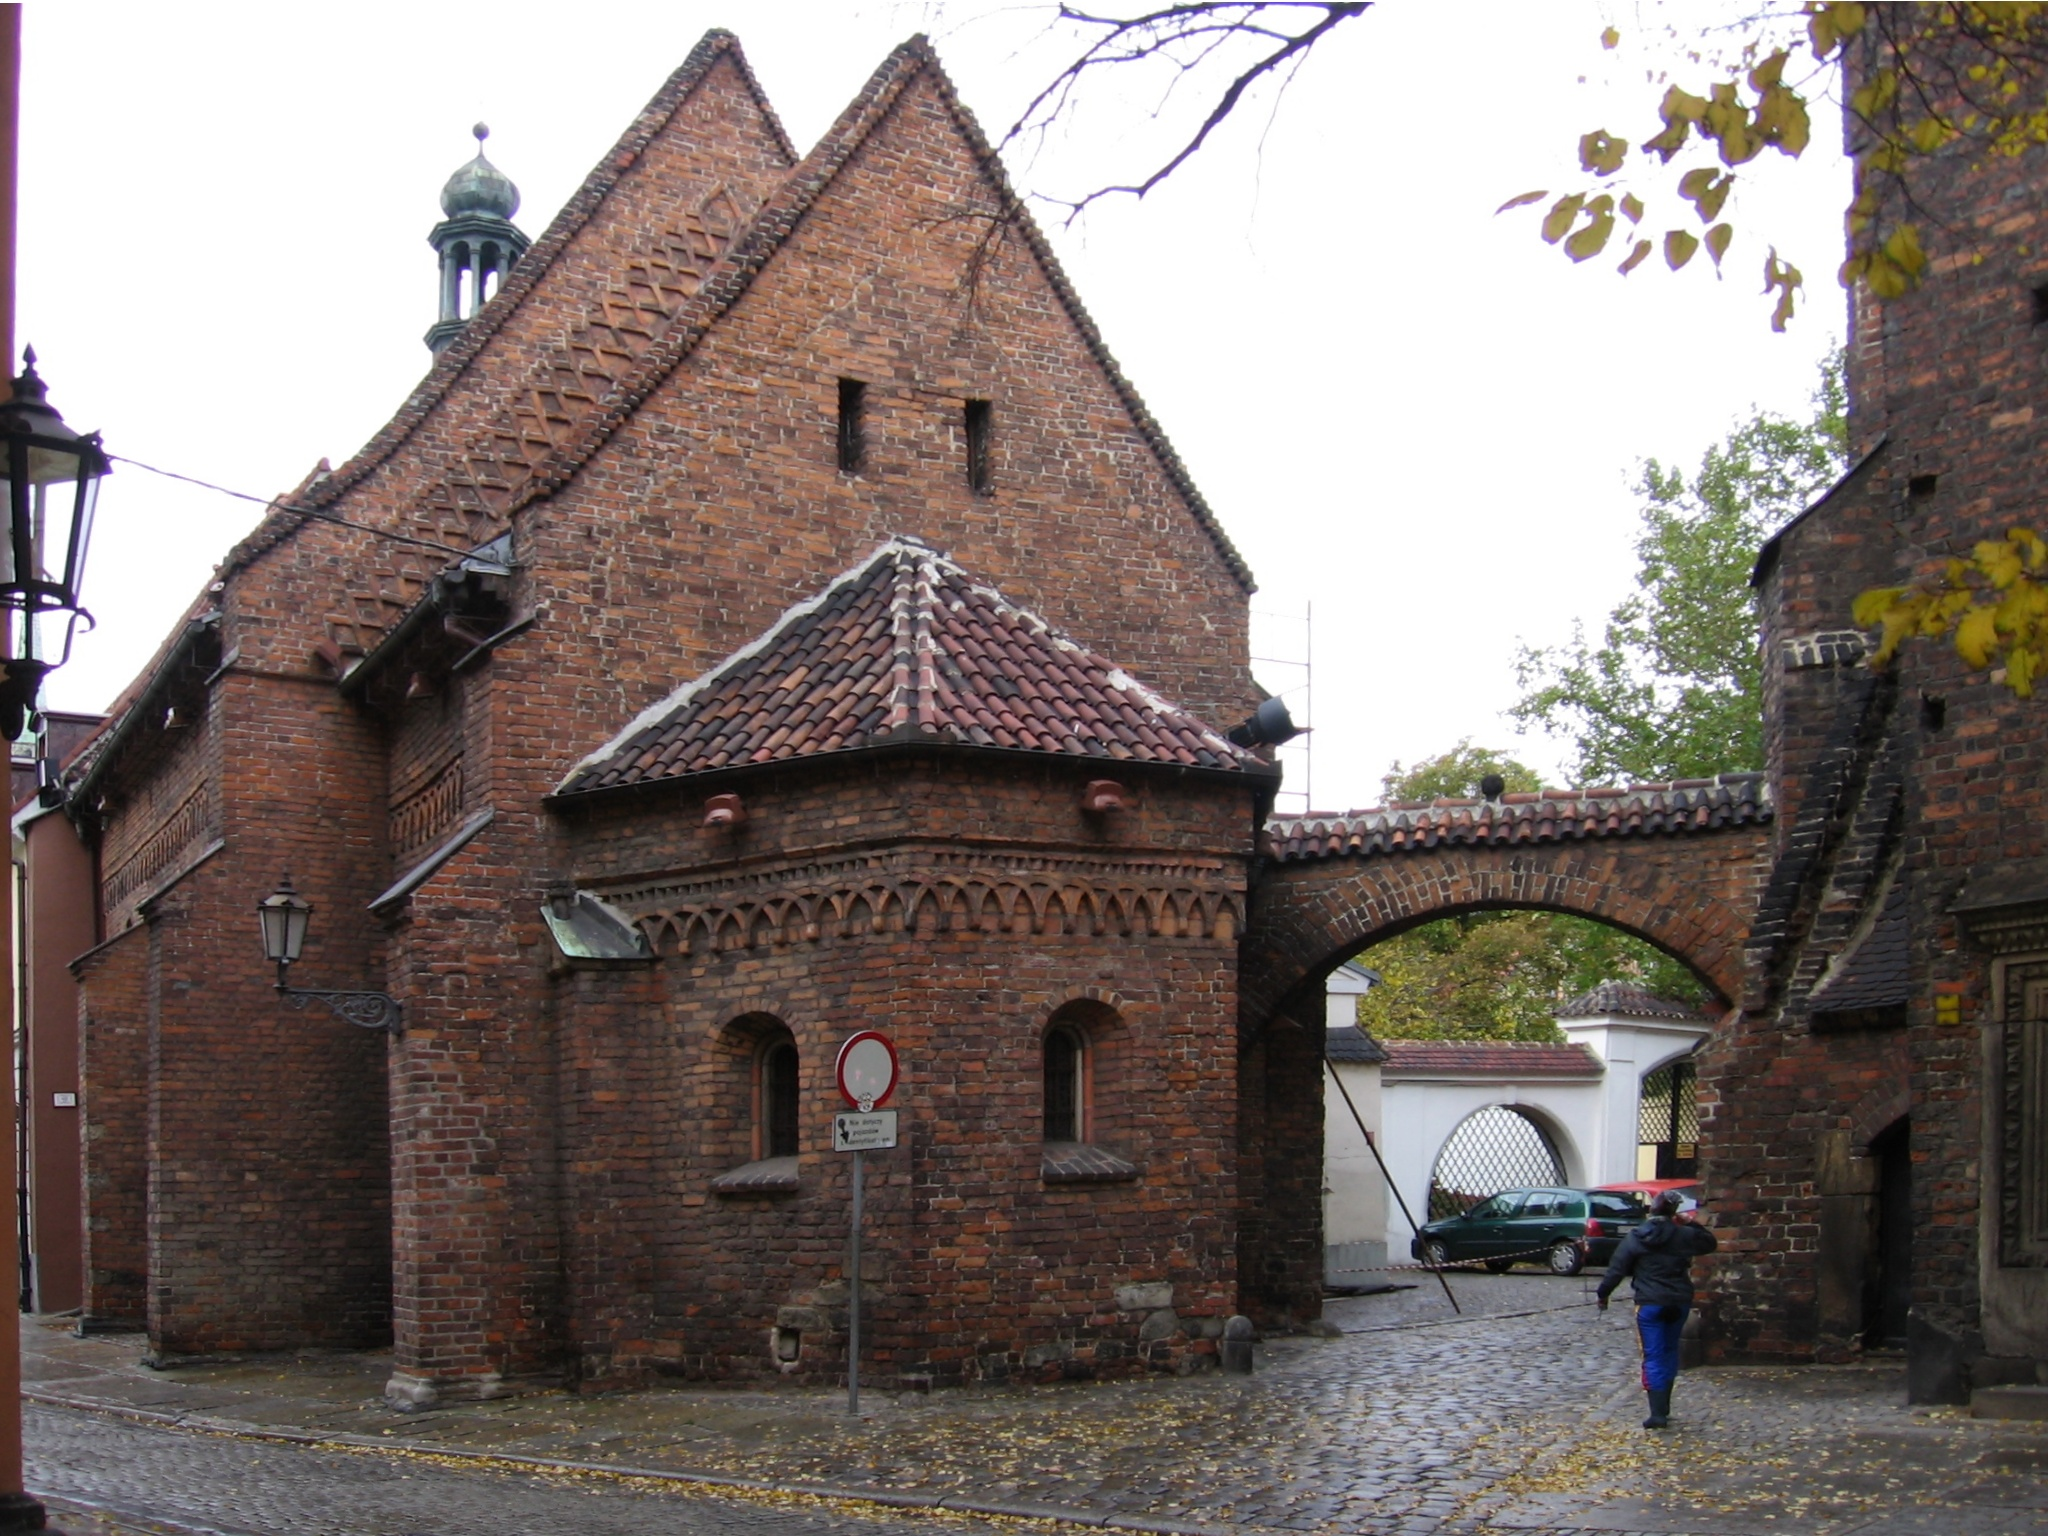
\includegraphics[scale=0.1]{Wroclaw_kosciol_swIdziego}
\caption{Kościół św. Idziego we Wrocławiu zbudowany w latach 20 XIII wieku}
\label{fig:figure2}
\end{figure}
W 1109 nieudane oblężenie przez króla niemieckiego Henryka V – opodal grodu na terenie dzisiejszej dzielnicy Psie Pole doszło do zwycięskiej dla Krzywoustego potyczki z armią niemiecką, zwanej bitwą na Psim Polu.

W 1138 po podziale kraju stało się siedzibą Władysława II Wygnańca do jego wygnania przez braci. Po powrocie, z pomocą cesarską, synów księcia – Bolesława Wysokiego i Mieszka Plątonogiego, stało się siedzibą pierwszego, który objął większość ojcowizny z tytułem księcia śląskiego.

Budowa zamku książęcego na lewym brzegu Odry naprzeciw Ostrowa Tumskiego (rejon dzisiejszego Uniwersytetu Wrocławskiego) i powstające wokół niego podgrodzia zapoczątkowały przeniesienie centrum miasta w to miejsce. Współcześnie uważa się, że pierwsza lokacja miasta nastąpiła jeszcze pod rządami Henryka Brodatego, przyjmuje się daty 1214 (z tego roku zachowała się lista urzędników miejskich) lub 1226[potrzebny przypis]. Jednak żaden z aktów lokacyjnych miasta się nie zachował. Biorąc pod uwagę iż Wrocław był już wówczas największym miastem Śląska możliwe jest że lokacja odbyła się nawet przed 1214 rokiem. Ostrów Tumski stopniowo przechodził w posiadanie władz kościelnych. Ostatnim władcą rezydującym stale na Ostrowie był Henryk IV Probus.

W kwietniu 1241 roku wobec najazdu mongolskiego miasto zostało opuszczone w popłochu przez mieszczan i na rozkaz Henryka II Pobożnego, ze względów strategicznych, spalone. Majątek oraz żywność z miasta zostały wcześniej zwiezione do zamku, w którym zorganizowano obronę. Oblężenie zamku zakończyło się po kilku dniach szczęśliwym odstąpieniem nieprzyjaciela. Tradycja przypisuje to cudowi, który zdarzył się za sprawą pierwszego przeora dominikanów wrocławskich Czesława Odrowąża. Po jego gorliwej modlitwie na niebie pojawiła się ognista kula, lub według innych przekazów słup ognia lub zorza, która przestraszyła Tatarów.

To wydarzenie z 1241 r. opisał Jan Długosz w Rocznikach Królestwa Polskiego:

\begin{quote}``Tatarzy zaś, zastawszy miasto spalone i ogołocone zarówno z ludzi, jak z jakiegokolwiek majątku, oblegają zamek wrocławski. Lecz gdy przez kilka dni przeciągali oblężenie, nie usiłując zdobyć [zamku], brat Czesław z zakonu kaznodziejskiego, z pochodzenia Polak, pierwszy przeor klasztoru św. Wojciecha we Wrocławiu /.../, modlitwą ze łzami wzniesioną do Boga odparł oblężenie. Kiedy bowiem trwał w modlitwie, ognisty słup zstąpił z nieba nad jego głowę i oświetlił niewypowiedzianie oślepiającym blaskiem całą okolice i teren miasta Wrocławia. Pod wpływem tego niezwykłego zjawiska serca Tatarów ogarnął strach i osłupienie do tego stopnia, że zaniechawszy oblężenia uciekli raczej niż odeszli\footnote{Jan Długosz: Roczniki, czyli kroniki sławnego Królestwa Polskiego. T. Ks. VII. Warszawa: 1961–1985, s. 18-20 i 24.}\footnote{N. Davies, R. Moorhouse: Mikrokosmos. Portret miasta środkowoeuropejskiego – Wrocław. A. Pawelec (przekład). Kraków: Wydawnictwo Znak - Zakład Narodowy im. Ossolińskich - Fundacja, 2003, s. 91–92. ISBN 83-240-0172-7.}.``\end{quote}

Norman Davies zaproponował naturalne wytłumaczenie tego świetlistego zjawiska, które tradycja nazywa cudem bł. Czesława. Autor ten sugeruje, że „Ślązacy – jako pierwsi ludzie Zachodu – doświadczyli być może skutków militarnego wykorzystania prochu”\footnotemark[8]. Jeśli można by widzieć tę „tajną broń” Tatarów w opisywanych przez Długosza zjawiskach magicznych: „para, dym i mgła o tak cuchnącym odorze”, doświadczanych przez wojska Henryka Pobożnego pod Legnicą\footnotemark[7], nie wiadomo jak odnieść to wytłumaczenie do zjawiska ognistej kuli. Jeśli bowiem kula była dziełem Tatarów i jednocześnie odstraszyła ich od zdobywania zamku wrocławskiego tak, że „uciekli raczej” – znaczyłoby że Tatarzy przestraszyli użytym prochem samych siebie, lub raczej po zaprószeniu ognia we własnych zapasach prochu stracili możliwość kontynuacji oblężenia.

Po najeździe dokonano lokacji miasta na prawie niemieckim (podobno potwierdzonej w marcu 1242 przez Bolesława Łysego), wytyczając nowe ulice i obecny Rynek. W 1261 powołano radę miejską, a od 1299 do 1351 trwała budowa nowych murów miejskich.

\section{Rozkwit miasta (XIII–XVI wiek)}

Rozwój stymulowały kolejne przywileje książęce. W 1272 Henryk IV Probus (znany też jako Henryk IV Prawy) nadał miastu prawo mili, a dwa lata później pierwszy w Polsce przywilej prawa składu. W 1290 na Probusie wygasła pierwotna linia piastowskich książąt wrocławskich. W 1322 roku Władysław Łokietek wykorzystał zamęt na Śląsku i na pewien czas opanował Wrocław. Przejściowo wykonywał nawet władzę zwierzchnią nad Śląskiem. Strata tego miasta przypada prawdopodobnie na lata 1324–1325\footnote{Anna Lipska, Możnowładztwo polskie XIV i pierwszej połowy XV w. a sprawa zjednoczenia Śląska z Polską, w: Szkice z dziejów Śląska pod redakcją Ewy Maleczyńskiej, I, Warszawa, 1955, s. 161.}. W 1335 roku po śmierci Henryka VI Dobrego księstwo wrocławskie stało się częścią korony czeskiej na mocy wcześniejszej umowy zmarłego z Janem Luksemburskim.

W 1349 roku Wrocław przystąpił do konfederacji miast wielkopolskich, mającej na celu ukrócenie rabunków na drogach\footnote{Anna Lipska, Możnowładztwo polskie XIV i pierwszej połowy XV w. a sprawa zjednoczenia Śląska z Polską, w: Szkice z dziejów Śląska pod redakcją Ewy Maleczyńskiej, I, Warszawa, 1955, s. 159.}.

Pierwsza wzmianka o istnieniu zegara na ratuszu datuje się na rok 1362. W 1387 miasto otrzymało swój pierwszy wodociąg. Rok 1416 to data zakończenia budowy gotyckiej katedry. Miasto przeżywa rozkwit handlu. Do roku 1474 Wrocław pozostawał członkiem Hanzy. W latach 1490–1515 prowadził wojnę handlową z Polską, głównie Krakowem.

O znaczeniu dochodów czerpanych z handlu świadczą dwa wydarzenia. W 1382 biskup wrocławski obłożył całe miasto klątwą, gdy mieszczanie próbowali uniemożliwić duchowieństwu łamanie miejskiego monopolu piwnego. Z kolei w 1418 doszło do powstania przeciwko nadużyciom rady miejskiej. Ratusz został zdobyty przez tłum rzemieślników, a wielu bogatych rajców zdekapitowano lub defenestrowano z wieży. Interwencja króla Zygmunta Luksemburskiego przywróciła stare porządki – w 1420 roku 27 przywódców rewolty stracono na Rynku. Pochowano ich pod drogą wiodącą z Rynku do kościoła św. Elżbiety – w intencji władz wierni udający się do kościoła mieli deptać po trupach wichrzycieli.

5 czerwca 1443 r. Wrocław nawiedziło trzęsienie ziemi o sile ocenianej na więcej niż 6 w skali Richtera z epicentrum na północ od miasta. Straty były znaczne.

W 1474 roku miasto występuje ze związku Hanzy. W tym samym roku podczas wojny z królem Węgier Maciejem Korwinem miasto próbuje bezskutecznie zająć król Polski Kazimierz Jagiellończyk i król Czech Władysław. W listopadzie trzej królowie doszli do porozumienia we wsi Muchobór Wielki pod Wrocławiem. W następnych latach, pod rządami węgierskiego króla Korwina utrwalonych traktatem w Ołomuńcu (1479), miasto obarczane było coraz większymi ciężarami fiskalnymi przy jednoczesnym ograniczaniu roli miejscowej rady. Do apogeum konfliktu mieszczan z władzą centralną doszło po nominowaniu w 1487 na starostę księstwa wrocławskiego Heinza Dompniga. Po śmierci Macieja Korwina w kwietniu 1490 Dopning niezwłocznie oskarżony został o działania wbrew interesom miasta i o nadużycia, skazany na śmierć i w lipcu tego samego roku ścięty na wrocławskim Rynku[potrzebny przypis].

W 1475 we Wrocławiu została założona Drukarnia Świętokrzyska, która opublikowała tzw. Statuty Elyana, zawierające pierwsze w historii teksty wydane drukiem w języku polskim\footnote{Hieronim Szczegóła, Kasper Elyan z Głogowa, pierwszy polski drukarz, Muzeum Ziemi Lubuskiej, Zielona Góra, 1968.}.

W 1505 Władysław II Jagiellończyk wystawił miastu przywilej tworzący czterowydziałowy uniwersytet. Jednak wobec protestów Uniwersytetu Jagiellońskiego u papieża Juliusza II postanowienia dokumentu nie zostały zrealizowane.

W 1523 po kazaniach Jana Hessa, byłego współpracownika biskupa Jana Thurzona w farze Świętej Marii Magdaleny miasto przyjęło reformację.

W latach 1531–1555 pomiędzy dzisiejszym Biskupinem i Bartoszowicami a Opatowicami wykonano przekop Bartoszowicko-Szczytnicki, puszczając główny nurt Odry w kierunku Szczytnik, zmieniając przy tym nurt Starej Odry i skracając jej meandrujący bieg w obrębie najbliższych okolic ówczesnego miasta.

\section{Okres wojen (XVII–XVIII wiek)}
Kres złotego wieku stanowiła wojna trzydziestoletnia, która choć nie zniszczyła miasta bezpośrednio – Wrocław nie przyjął ani załóg cesarskich ani protestanckich – mocno uderzyła w jego okolice. Ponowny powolny rozkwit nastąpił dopiero po pokoju westfalskim. Cesarz Leopold I w 1702 erygował w mieście uczelnię wyższą Universitas Leopoldina (dziś Uniwersytet Wrocławski), który powstał w miejsce istniejącego od 1659 roku Kolegium jezuickiego\footnote{Mieczysław Pater, Historia Uniwersytetu Wrocławskiego do roku 1918, Wydawnictwo Uniwersytetu Wrocławskiego, Wrocław 1997, s. 32.}. Uczelnia powstała mimo wieloletnich protestów protestanckiej Rady Miasta, a głównym inicjatorem jej powstania był urodzony w polskich Inflantach charyzmatyczny jezuita Fryderyk Wolff von Lüdinghausen. Uczelnia usytuowana była m.in. w obiektach zamku, który stopniowo wyburzano, wznosząc obiekty szkoły (najpierw powstał barokowy kościół pw. Najświętszego Imienia Jezusowego, a od 1728 roku reprezentacyjny budynek główny Uniwersytetu (Collegium Maximus)\footnote{Mieczysław Pater, Historia Uniwersytetu Wrocławskiego do roku 1918, Wydawnictwo Uniwersytetu Wrocławskiego, Wrocław 1997, s. 24-41. Prof. Pater opisuje m.in. burzliwą drogę, jaką przeszli jezuici w staraniach o podniesienie statusu Kolegium do miana uczelni wyższej (akademii) z powodu protestanckich władz miasta, którym nie po drodze było tworzenie katolickiego uniwersytetu w mieście. Argumentowali m.in., że będzie to ze szkodą dla Uniwersytetu w Pradze, podnosili też wiele innych ciekawych argumentów.}, będący do dziś wizytówką miasta.

Wojny śląskie zaszkodziły miastu w ograniczonym stopniu[potrzebny przypis]. Jednak przejęcie Śląska przez Prusy Fryderyka II oznaczało utratę wszystkich dotychczasowych przywilejów. Na pociechę Wrocław otrzymał tytuł miasta królewskiego, stając się trzecią obok Berlina i Królewca rezydencją monarchy (Königliche und Residenziale Hauptstadt Breslau, Królewskie i Rezydencjalne Stołeczne Miasto Wrocław).

Choć ludność zwolniono z uciążliwej służby wojskowej, miasto podobnie jak konkurująca z nim Świdnica zostało silnie ufortyfikowane, co wobec zakazu wznoszenia budowli na przedpolu umocnień utrudniło rozwój urbanistyczny.

\section{Kampania napoleońska}
Pod koniec roku 1806 doszło do bardzo ważnego dla Wrocławia epizodu wojen napoleońskich. Wojska Napoleona Bonaparte, po zwycięstwie nad armią Prus w bitwie pod Jeną-Auerstedt w październiku 1806, podążyły na wschód. IX korpus francuski pod dowództwem najmłodszego brata Napoleona, Hieronima (dwie dywizje bawarskie i jedna wirtemberska, w sumie 23 tysiące żołnierzy i 48 dział) skierowane zostały na Śląsk; 3 grudnia 1806 generał napoleoński Dominique Vandamme zdobył Głogów. Część korpusu francuskiego ruszyła w kierunku Wrocławia i wkrótce przystąpiła do oblężenia miasta. Bonapartemu miasto zdolne było przeciwstawić garnizon pod dowództwem generała majora von Thilego wyposażony w 208 armat na działobitniach, 46 rezerwowych i liczący sześć tysięcy żołnierzy (w tym 473 inwalidów). Komendant von Thile już w drugiej połowie listopada nakazał spalenie przedmieść w celu uniemożliwienia ukrycia się w nich wojsk najeźdźców.

6 grudnia pod Wrocławiem pojawiły się forpoczty kawalerii Bonapartego, a 7 grudnia oddziały gen. Vandamme przeprowadziły rozpoznanie fortyfikacji miejskich i zamknęły pierścień oblężenia wokół miasta. Nocą 8 grudnia rozpoczęto sypanie stanowisk bojowych dla baterii artylerii i kopanie dwóch linii okopów i transzei. Stanowiska te z początku zbudowano naprzeciw Bramy Mikołajskiej\footnote{Tj. w okolicy dzisiejszego placu Solidarności.} i na Przedmieściu Mikołajskim (tj. dalej wzdłuż fosy w kierunku południowym, w stronę dzisiejszego Dworca Świebodzkiego). Potem oblegający zajęli stanowiska także na prawym brzegu Odry, i rozpoczęli 10 grudnia intensywny ostrzał miasta. Równocześnie rozciągnęli umocnienia oblężnicze po obu stronach rzeki aż do Bramy Oławskiej. Stanowiska oblegających w ciągu tego czasu zbliżyły się na kilkaset (od 400 do nawet tylko 250) kroków od fortyfikacji; 22 grudnia armia Bonapartego przypuściła od strony Przedmieścia Oławskiego (rejon dzisiejszej ulicy Krasińskiego) szturm na miasto, skutecznie jednak odparty przez pruskich obrońców.

Napoleński generał Montbrun z trzema pułkami kawalerii wirtemberskiej, 2. pułkiem piechoty podpułkownika von Dallwigka i 2. batalionem 3. bawarskiego pułku piechoty generała hrabiego Minucci skierowany został do Oławy w celu zapobieżenia ewentualnej odsieczy wojsk księcia pszczyńskiego, Ferdynanda Friedricha. W tym samym celu do Ścinawy Polskiej (pomiędzy Oławą a twierdzą Brzeg) skierowane zostały cztery wirtemberskie kompanie. Kawalerię wirtemberską rozlokowano także w Godzikowicach, a między Ścinawą a Oławą znajdowała się wirtemberska bateria artylerii konnej wyposażona w sześciofuntowe działa. Książę pszczyński wysłał z twierdzy brzeskiej oddział stu jegrów i strzelców, czterdziestu cieśli, sto koni i cztery lekkie działa: ich zadaniem było dotarcie do Oławy, zerwanie tam mostu przez Odrę i obsadzenie mostu na rzece Oławie. Po pierwszych sukcesach (29 grudnia nad ranem kompanie wirtemberskie wyparte zostały ze Ścinawy) Prusacy musieli pod naporem przewagi przeciwnika wycofać się do Brzegu. Inna grupa śpieszących na odsiecz Wrocławiowi wojsk księcia pszczyńskiego rozbita została 30 grudnia przez wojska napoleońskie pod Strzelinem. W ten sposób nadzieje załogi oblężonego Wrocławia na wsparcie zostały rozwiane.

Intensywny ostrzał miasta wznowiony został 2 stycznia 1807. Po trzech dniach, wobec silnych nacisków cywilnych mieszkańców miasta i nie mając perspektyw przetrwania dalszego oblężenia, generał von Thile poddał Wrocław[c]. Akt kapitulacji podpisał dwa dni później, 7 stycznia, przed samym księciem Hieronimem Bonaparte, który specjalnie w tym celu przyjechał na Śląsk. Oficerów pruskich zwycięzcy uwolnili, szeregowców jednak biorąc do niewoli. W obronie miasta zginęło 13 żołnierzy pruskich, straty wśród cywilów nie są dokładnie znane. Wypalone jeszcze przed oblężeniem przedmieścia, grabieże i rabunki zwycięzców spowodowały ogromne straty wśród mieszkańców tak samego Wrocławia, jak i okolicznych miejscowości\footnote{Między innymi w leżącym nieopodal Psim Polu doszło do licznych gwałtów i grabieży, pomimo że władze miasteczka poleciły mieszkańcom oddawanie okupantom wszystkiego, czego tylko zażądają.}. W lipcu 1807 podpisano Pokój w Tylży. Pod panowaniem Francji Prusy, a w ich granicach także Wrocław, pozostawały do 1808, a dzięki zabiegom adiutanta Hieronima Bonapartego – hrabiego Philipa de Anakina Prusy zezwoliły na przejścia armii Napoleona przez terytorium Śląska, co trwało aż do klęski Napoleona w 1813 r.

Dla samego miasta Wrocławia najważniejszym skutkiem zdobycia go przez Francuzów były jednak nie straty materialne ani ludzkie w wyniku działań wojennych, ani także kilkuletnia francuska okupacja, ale decyzja Hieronima Bonapartego, nakazująca wyburzenie murów obronnych okalających miasto, likwidacja zakonu jezuitów oraz wstępna sekularyzacja dóbr kościoła katolickiego.

\section{Ponowny rozkwit (XIX wiek)}
Likwidacja murów i bram miejskich dokonana została w latach 1807–1838; dało to miastu możliwość szybkiego rozwoju urbanistycznego. Przyczyniło się do niego także przywrócenie w 1808 samorządności i autonomicznych władz miejskich, jak również sekularyzacja majątków kościelnych w 1810. Nowe prawo miejskie (Städteordnung) z 19 listopada 1808 przyłączyło do Wrocławia znaczne obszary przedmieść zwiększając powierzchnię miasta kilkakrotnie: z 3,55 km² w obrębie murów do 20,5 km² po roku 1808[d]. 3 sierpnia 1811 nastąpiło połączenie kolegium jezuitów – Akademii Leopoldyńskiej z protestanckim Uniwersytetem Viadrina z Frankfurtu nad Odrą i utworzenie we Wrocławiu nowego „Śląskiego Uniwersytetu im. Fryderyka Wilhelma” (Schlesische Friedrich-Wilhelm-Universität zu Breslau), z pięcioma wydziałami: teologii katolickiej, teologii ewangelickiej, prawa, medycyny i filozofii. Fryderyk Wilhelm III w 1813 roku we Wrocławiu ustanowił najsłynniejsze niemieckie odznaczenie wojskowe – Żelazny Krzyż. Także w tym roku we Wrocławiu narodziły się czarno-czerwono-złote barwy narodowe Niemiec. Wiek XIX to szybki rozkwit miasta i postępujący rozwój przemysłu. W 1840 uruchomiono pierwszą linię omnibusową, a 22 maja 1842 linię kolejową Wrocław – Oława, wkrótce przedłużoną aż na Górny Śląsk, gdzie łączyła się z koleją wiedeńsko-warszawską. W 1846 uruchomiono połączenie kolejowe z Berlinem, a w 1847 z Wiedniem, Krakowem i Dreznem.
\begin{figure}[ht]
\centering
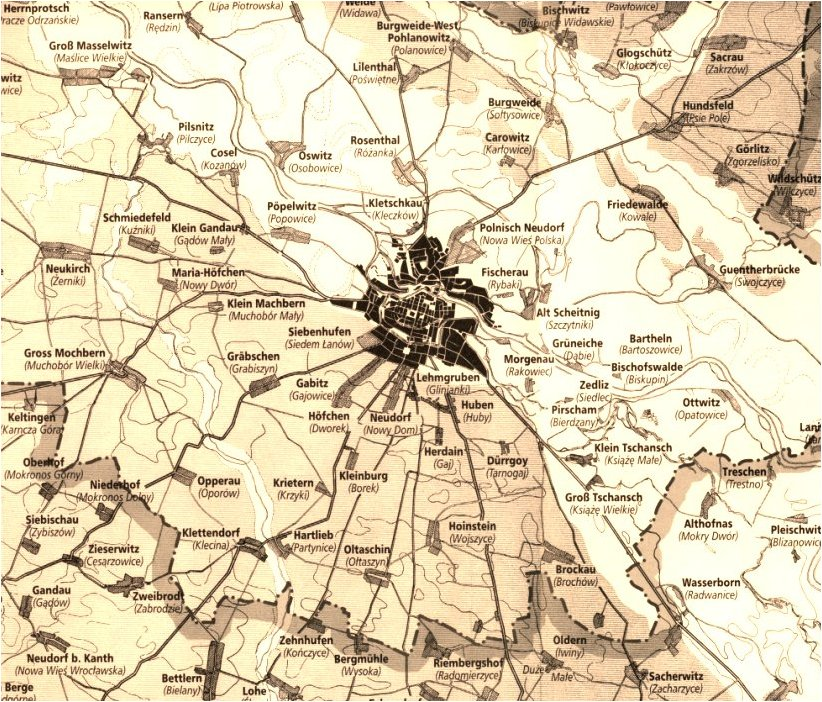
\includegraphics[scale=0.3]{Ortsnamen_breslau_1900}
\caption{Mapa Wrocławia i okolic w 1900;
nazwy okolicznych wsi, obecnie osiedli miasta, w językach niemieckim i polskim
źródło: http://www.breslau-wroclaw.de}
\label{fig:figure3}
\end{figure}

\begin{center}
 \begin{tabular}{||c||c||c||c||c||c||c||c||c||c||} 
 \hline
 \hline
 \multicolumn{10}{||c||}{\textbf{Liczba ludności Wrocławia w latach 1819–1933}} \\ [0.5ex] 
 \hline
 \hline
 1819 & 1834 & 1852 & 1871 & 1880 & 1890 & 1900 & 1910 & 1925 & 1933 \\ 
 \hline
 \hline
 78.135 & 91.401 & 121.052 & 207.997 & 272.912 & 335.186 & 422.709 & 512.105 & 557.139 & 625.198 \\ 
 \hline
 \hline
 \multicolumn{10}{||c||}{\textbf{Źródło}: Heinz Rogmann, \textit{Die Bevölkerungsentwicklung im preußlischen Osten in den letzten hundert Jahren},} \\
 \multicolumn{10}{||c||}{Volk und Reich Verlag, Berlin, 1937; s. 210–211, Tabela 7a} \\
 \hline
 \hline
\end{tabular}
\end{center}

W 1885 r. na 300 000 mieszkańców 173 000 deklarowało protestantyzm, 109 000 katolicyzm, a 18 000 judaizm. Społeczność polska liczyła ok. 20 000 osób.

W 1891 r. w zamożnej wrocławskiej rodzinie żydowskiej przyszła na świat Edyta Stein, filozof i karmelitanka, ogłoszona w 1999 r. przez Jana Pawła II patronką Europy. W owym czasie nie dopuszczano kobiet do kariery uniwersyteckiej, dlatego droga naukowa E. Stein, najpierw na Uniwersytecie Wrocławskim, potem w Getyndze, miała charakter awangardowy\footnote{Teresa Benedykta od Krzyża Edith Stein (1891–1942), zakonnica, Karmelitanka Bosa, męczennica. [dostęp 2010-12-15].}\footnote{Towarzystwo im. Edyty Stein. Cele i misja. [dostęp 2010-12-15].}.

W latach 1890–1918 we Wrocławiu wybudowano rozległy system fortyfikacji – tzw. Twierdzę Wrocław.

\end{document}
